%%% Copyright (C) 2020 Vincent Goulet
%%%
%%% Ce fichier fait partie du projet
%%% «Rédaction avec LaTeX»
%%% https://gitlab.com/vigou3/formation-latex-ul
%%%
%%% Cette création est mise à disposition sous licence
%%% Attribution-Partage dans les mêmes conditions 4.0
%%% International de Creative Commons.
%%% https://creativecommons.org/licenses/by-sa/4.0/

\section{Et la suite?}

\begin{frame}
  \frametitle{Pour en savoir plus}

  \begin{columns}
    \begin{column}{.6\textwidth}
      Le document de référence fournit des détails additionnels et
      couvre des concepts plus avancés:
      \begin{itemize}
        \small
      \item boites, tableaux et figures
      \item équations mathématiques élaborées
      \item bibliographie et citations
      \item commandes et environnement sur mesure
      \item changement de police
      \item diapositives
      \item etc.
      \end{itemize}
    \end{column}
    \begin{column}{.4\textwidth}
      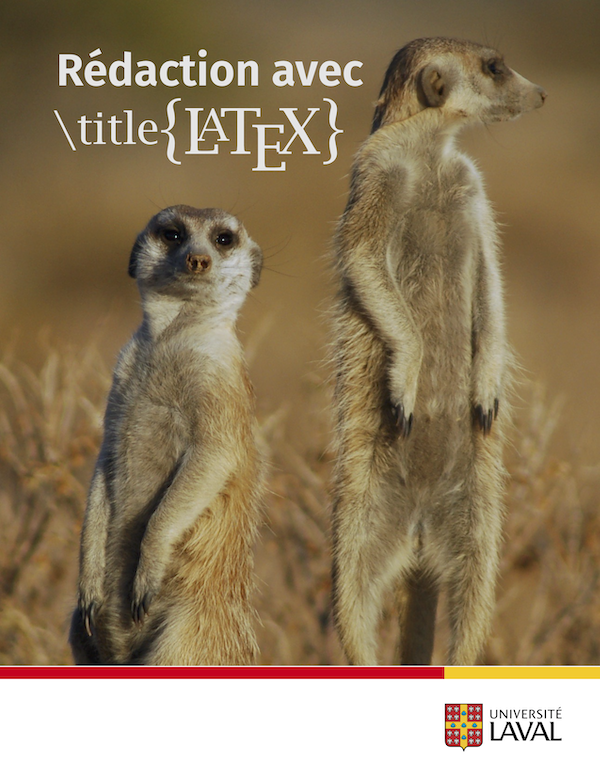
\includegraphics[height=0.8\textheight,frame]{images/formation-latex-ul}
    \end{column}
  \end{columns}
\end{frame}

%%% Local Variables:
%%% TeX-master: "formation-latex-ul-diapos"
%%% TeX-engine: xetex
%%% coding: utf-8
%%% End:
